%%%%%%%%%%%%%%%%%%%%%%%%%%%%%%%%%%%%%%%%%%%%%%%%%%%%%%%%%%%%%%%%%%%%%%%%%%%%%%%%%%%%%%%%%%%%%%%%%
%
% Document:     DM Support Prd.
  product tree
%
%%%%%%%%%%%%%%%%%%%%%%%%%%%%%%%%%%%%%%%%%%%%%%%%%%%%%%%%%%%%%%%%%%%%%%%%%%%%%%
\documentclass{article}
\usepackage{times,layouts}
\usepackage{tikz,hyperref,amsmath}
\usetikzlibrary{positioning,arrows,shapes,decorations.shapes,shapes.arrows}
\usetikzlibrary{backgrounds,calc}
\usepackage[paperwidth=57.2cm,paperheight=14.540000000000001cm,
left=-2mm,top=3mm,bottom=0mm,right=0mm,
noheadfoot,marginparwidth=0pt,includemp=false,
textwidth=30cm,textheight=50mm]{geometry}
\newcommand\showpage{%
\setlayoutscale{0.5}\setlabelfont{\tiny}\printheadingsfalse\printparametersfalse
\currentpage\pagedesign}
\hypersetup{pdftitle={DM products }, pdfsubject={Diagram illustrating the
                products in LSST DM }, pdfauthor={Autogenerated from MD}}
\tikzstyle{tbox}=[rectangle,text centered, text width=30mm]
\tikzstyle{wbbox}=[rectangle, rounded corners=3pt, draw=black, top color=blue!50!white,
                    bottom color=white, very thick, minimum height=12mm, inner sep=2pt,
                    text centered, text width=30mm]
\tikzstyle{pbox}=[rectangle, rounded corners=3pt, draw=black, top
 color=yellow!50!white, bottom color=white, very thick,
 minimum height=35pt, inner sep=2pt, text centered, text width=35mm]
\tikzstyle{pline}=[-, thick]
\begin{document}
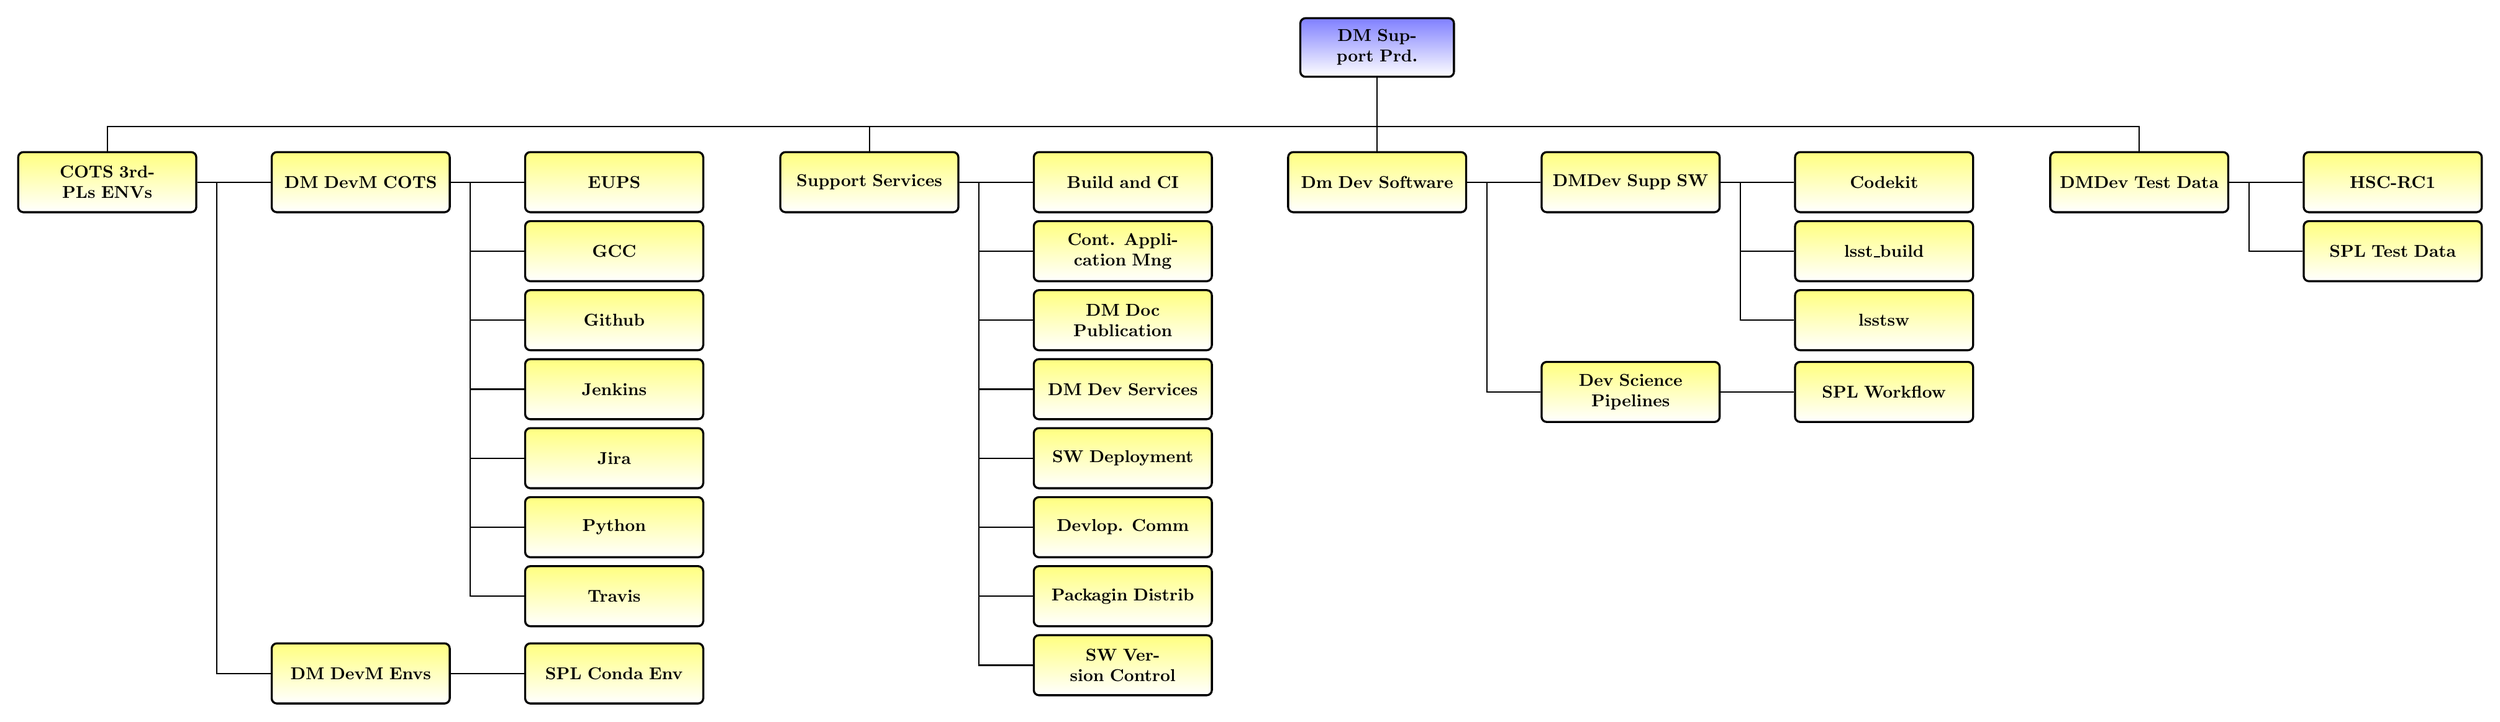
\begin{tikzpicture}[node distance=0mm]


\node (DMDC3E) [pbox, 
] {\textbf{COTS 3rdPLs ENVs
} };
\node (COTSDM) [pbox,right=15mm of DMDC3E] {\textbf{DM DevM COTS
} };
 \draw[pline] (DMDC3E.east) -| ++(0.4,0) |- (COTSDM.west); 
\node (EUPS) [pbox,right=15mm of COTSDM] {\textbf{EUPS
} };
 \draw[pline] (COTSDM.east) -| ++(0.4,0) |- (EUPS.west); 
\node (GCC) [pbox,below=4pt of EUPS] {\textbf{GCC
} };
 \draw[pline] (COTSDM.east) -| ++(0.4,0) |- (GCC.west); 
\node (GITHUB) [pbox,below=4pt of GCC] {\textbf{Github
} };
 \draw[pline] (COTSDM.east) -| ++(0.4,0) |- (GITHUB.west); 
\node (JNKNS) [pbox,below=4pt of GITHUB] {\textbf{Jenkins
} };
 \draw[pline] (COTSDM.east) -| ++(0.4,0) |- (JNKNS.west); 
\node (JRA) [pbox,below=4pt of JNKNS] {\textbf{Jira
} };
 \draw[pline] (COTSDM.east) -| ++(0.4,0) |- (JRA.west); 
\node (PTHN) [pbox,below=4pt of JRA] {\textbf{Python
} };
 \draw[pline] (COTSDM.east) -| ++(0.4,0) |- (PTHN.west); 
\node (TRVS) [pbox,below=4pt of PTHN] {\textbf{Travis
} };
 \draw[pline] (COTSDM.east) -| ++(0.4,0) |- (TRVS.west); 
\node (DENV) [pbox,below=250pt of COTSDM] {\textbf{DM DevM Envs
} };
 \draw[pline] (DMDC3E.east) -| ++(0.4,0) |- (DENV.west); 
\node (SPLCE) [pbox,right=15mm of DENV] {\textbf{SPL Conda Env
} };
 \draw[pline] (DENV.east) -| ++(0.4,0) |- (SPLCE.west); 
\node (DMDSRV) [pbox, 
right=11.9cm of DMDC3E] {\textbf{Support Services
} };
\node (BCI) [pbox,right=15mm of DMDSRV] {\textbf{Build and CI
} };
 \draw[pline] (DMDSRV.east) -| ++(0.4,0) |- (BCI.west); 
\node (CAM) [pbox,below=4pt of BCI] {\textbf{Cont. Application Mng
} };
 \draw[pline] (DMDSRV.east) -| ++(0.4,0) |- (CAM.west); 
\node (DDCPUB) [pbox,below=4pt of CAM] {\textbf{DM Doc Publication
} };
 \draw[pline] (DMDSRV.east) -| ++(0.4,0) |- (DDCPUB.west); 
\node (DDVSRV) [pbox,below=4pt of DDCPUB] {\textbf{DM Dev Services
} };
 \draw[pline] (DMDSRV.east) -| ++(0.4,0) |- (DDVSRV.west); 
\node (DEPLOY) [pbox,below=4pt of DDVSRV] {\textbf{SW Deployment
} };
 \draw[pline] (DMDSRV.east) -| ++(0.4,0) |- (DEPLOY.west); 
\node (DMDCOM) [pbox,below=4pt of DEPLOY] {\textbf{Devlop. Comm
} };
 \draw[pline] (DMDSRV.east) -| ++(0.4,0) |- (DMDCOM.west); 
\node (PKGDST) [pbox,below=4pt of DMDCOM] {\textbf{Packagin Distrib
} };
 \draw[pline] (DMDSRV.east) -| ++(0.4,0) |- (PKGDST.west); 
\node (SWVER) [pbox,below=4pt of PKGDST] {\textbf{SW Version Control
} };
 \draw[pline] (DMDSRV.east) -| ++(0.4,0) |- (SWVER.west); 
\node (DMDSW) [pbox, 
right=6.7cm of DMDSRV] {\textbf{Dm Dev Software
} };
\node (DMDSS) [pbox,right=15mm of DMDSW] {\textbf{DMDev Supp SW
} };
 \draw[pline] (DMDSW.east) -| ++(0.4,0) |- (DMDSS.west); 
\node (CDKT) [pbox,right=15mm of DMDSS] {\textbf{Codekit
} };
 \draw[pline] (DMDSS.east) -| ++(0.4,0) |- (CDKT.west); 
\node (LBLD) [pbox,below=4pt of CDKT] {\textbf{lsst\_build
} };
 \draw[pline] (DMDSS.east) -| ++(0.4,0) |- (LBLD.west); 
\node (LSSTSW) [pbox,below=4pt of LBLD] {\textbf{lsstsw
} };
 \draw[pline] (DMDSS.east) -| ++(0.4,0) |- (LSSTSW.west); 
\node (DSPLSW) [pbox,below=86pt of DMDSS] {\textbf{Dev Science Pipelines
} };
 \draw[pline] (DMDSW.east) -| ++(0.4,0) |- (DSPLSW.west); 
\node (SPLWF) [pbox,right=15mm of DSPLSW] {\textbf{SPL Workflow
} };
 \draw[pline] (DSPLSW.east) -| ++(0.4,0) |- (SPLWF.west); 
\node (DMDTD) [pbox, 
right=11.9cm of DMDSW] {\textbf{DMDev Test Data
} };
\node (HSCRC1) [pbox,right=15mm of DMDTD] {\textbf{HSC-RC1
} };
 \draw[pline] (DMDTD.east) -| ++(0.4,0) |- (HSCRC1.west); 
\node (SPLTD) [pbox,below=4pt of HSCRC1] {\textbf{SPL Test Data
} };
 \draw[pline] (DMDTD.east) -| ++(0.4,0) |- (SPLTD.west); 
\node (DMDEV) [wbbox, above=15mm of DMDSW]{\textbf{DM Support Prd.
}};
 \draw[pline]   (DMDC3E.north) -- ++(0.0,0.5) -| (DMDEV.south) ; 
 \draw[pline]   (DMDSRV.north) -- ++(0.0,0.5) -| (DMDEV.south) ; 
 \draw[pline]   (DMDSW.north) -- ++(0.0,0.5) -| (DMDEV.south) ; 
 \draw[pline]   (DMDTD.north) -- ++(0.0,0.5) -| (DMDEV.south) ; 

\end{tikzpicture}
\end{document}
